
%\documentclass[useAMS,usenatbib]{mn2e}
\documentclass[useAMS,usenatbib]{mnras}
%\documentclass[usenatbib]{mn2e}
\usepackage{graphicx}
%\usepackage[nottoc]{tocbibind}
\setlength{\topmargin}{-1.2cm}

% If your system does not have the AMS fonts version 2.0 installed, then
% remove the useAMS option.
%
% useAMS allows you to obtain upright Greek characters.
% e.g. \umu, \upi etc.  See the section on "Upright Greek characters" in
% this guide for further information.
%
% If you are using AMS 2.0 fonts, bold math letters/symbols are available
% at a larger range of sizes for NFSS release 1 and 2 (using \boldmath or
% preferably \bmath).
%
% The usenatbib command allows the use of Patrick Daly's natbib.sty for
% cross-referencing.
%
% If you wish to typeset the paper in Times font (if you do not have the
% PostScript Type 1 Computer Modern fonts you will need to do this to get
% smoother fonts in a PDF file) then uncomment the next line
% \usepackage{Times}

%%%%% AUTHORS - PLACE YOUR OWN MACROS HERE %%%%%

% Journal definitions
%\newcommand{\apj}[1]{ApJ}
%\newcommand{\mnras}[1]{MNRAS}
%\newcommand{\apjl}[1]{ApJL}
%\newcommand{\pasj}[1]{PASJ}
%\newcommand{\aj}[1]{AJ}
%\newcommand{\nat}[1]{Nature}
%\newcommand{\aap}{A\&A}

%%%%%%%%%%%%%%%%%%%%%%%%%%%%%%%%%%%%%%%%%%%%%%%%

\title[Beware the Effect of Edge-on Disks]{
%Gravitational Lens Modelling of flux-ratio Anomalous System B1555+375
SHARP II: Dark Matter Substructure, Gravitational Lens flux-ratio
Anomalies, and the Case of B1555+375: Beware the Effect of Edge-on
Disks
}
\author[Hsueh et al.]{Jen-Wei Hsueh$^{1}$\thanks{E-mail:
jwhsueh@ucdavis.edu (JWH); otheremail@otheraddress (ANO)} and A. N.
Other$^{2}$\\
$^{1}$Physics Dept., University of California, Davis, 1 Shields Ave.
Davis, CA 95616, USA\\
$^{2}$Building, Institute, Street Address, City, Code, Country}
\begin{document}

%\date{Accepted 1988 December 15. Received 1988 December 14; in original form 1988 October 11}

\pagerange{\pageref{firstpage}--\pageref{lastpage}} \pubyear{2015}

\maketitle

\label{firstpage}

\begin{abstract}

Gravitational lens flux-ratio anomalies provide a powerful technique
for detecting the presence of dark matter substructure in distant
galaxies.  However, before using the statistics of systems with these
anomalies, it is imperative to ascertain that a given system does not
have properties that could plausibly cause the observed anomaly
without the need for substructure.  In this letter, we present the
case of the B1555+375 lens system, which has a strong radio-wavelength
flux-ratio anomaly but where the lensing galaxy is also revealed in
high-resolution infrared imaging to have a clear edge-on disk component.  The
disk crosses directly over the pair of images that exhibit the
anomaly, and we show that simple models that include the disk can
reproduce the anomaly without requiring substructure.  
%Other lens systems that we have observed with adaptive optics imaging
%as part of the Strong lensing at High Angular Resolution Programme (SHARP)
%show a similar behaviour and will be the subject of a future paper.  
These results suggest that the assumption that
all flux-ratio anomalies are due to substructure will likely overestimate
the substructure fraction in massive galaxies.

\end{abstract}

\begin{keywords}
gravitational lensing
\end{keywords}

\section{Introduction}

A common feature of simulations of structure formation is the presence
of thousands of subhaloes that are associated with larger mass haloes \citep[e.g.][]{Springel08}.
However, observations of the Local Group show many fewer satellite
galaxies than are predicted by the simulations, even when taking into
account completeness corrections arising from the limited sky coverage
imposed by the Galactic Plane and the latest discovery of new dwarf galaxies \citep{DES15,Kop15}.  
This is the famous ``missing satellite'' problem \citep{Klypin1999, Moore1999, S07}. In order to
understand this discrepancy, it is imperative to build up a large
sample of satellites/subhaloes in galaxies outside the Local Group.
 However, this process is challenging due to the faintness of the satellite
galaxies.  Furthermore, lower-mass satellites may not be able to
retain the gas needed for ongoing star formation \citep[e.g.][]{P11},
rendering them effectively dark.  These factors make gravitational
lensing a powerful and promising tool for the detection of
substructure.

It was first suggested by \citet{Mao1998} that flux-ratio anomalies
observed in radio-loud multiple images of lensed quasars could be
interpreted as a telltale sign of the presence of substructure in lens
galaxies.  Indeed, small perturbations in the gravitational potential
are sufficient to cause flux-ratio anomalies in strong lensed systems
\citep{Bradac02}.  Moreover, unlike in the optical or infrared, in the
radio band, lensed images are neither sensitive to microlensing from
stars, nor to dust extinction. This makes flux-ratio anomalies a promising
tool to detect \textbf{and measure} dark matter substructures \citep{Dalal2002,N13}.  
%At present, the amount of substructure derived from flux-ratio anomalies
%seems to be disagreement with predictions from numerical simulations, 
%with the former requiring a larger fraction of mass in substructure than
%expected \citep{Xu14}. 
\textbf{At present, the amount of substructures derived from flux-ratio anomalies eases the disagremeent with direct detections and numerical simulations.
\emph{Gravitational imaging technique}, by utilizing the surface brightness distribution of extended arcs and Einstein rings,
has been introduced by \citet{K05} and \citet{V09} and gives the measurements of the fraction of
substructure. The result
is currently in agreement with theoretical expectations \citep{V14a,V12} although the simulation results show less level of flux anomalies than expected \citep{Xu14}.}
While this could be the result of small sample
statistics, it could also be an indication that flux-ratio anomalies
have a different origin than substructure. \textbf{ISM and microlensing both can produce flux anomalies in strong lens systems, but not like substurcture pertubations, the effects from ISM show strong frequency dependence and  microlensing from star-size objects is negligible in radio band. These alternative origins have been ruled out among known radio loud flux anomlous systems which implies detection of substructures \citep{KD04}. }[OTHER POSSIBLE ORIGONS--SIMONA]
%


%While future large-scale surveys, such as the LSST, are expected to
%deliver new large samples of gravitationally lensed quasars, in the
%near future the discovery of new systems using narrow-line quasar
%emission \citep{N14} will provide new invaluable statistical
%perspective on current constraints based on flux-ratio anomalies.  
In this letter, we explore the idea that not all flux-ratio anomalies are
related to the presence of substructure, but that some originate in a
more complex lens galaxy mass distribution than initially
considered. To this end we use new infra-red data from the Strong
lensing at High Angular Resolution Program 
\citep[SHARP;][Fassnacht et al., in prep]{SHARP12, V12}.
The main goal of the SHARP project is to re-observe known
quadruple and Einstein ring lens systems at high angular
resolution by making use of observations with (1) adaptive optics (AO)
on the Keck telescopes, (2) the Hubble Space Telescope, and (3) large
interferometric arrays \citep{SHARP12,V12}. In particular, 
we focus on the B1555+375 lens system\citep{Marlow99} to better
understand the causes of flux-ratio anomalies in gravitational lenses.  This system was
discovered in the Cosmic Lens All-Sky Survey \citep{CLASS1,CLASS2} and
has a pair of merging images that show a strong \textbf{persistent} flux-ratio anomaly at
radio wavelengths.  Follow-up observations ruled out radio propagation
effects as the cause of the anomaly \citep{K03,KD04}.  The B1555+375
system was included in both the observational and theoretical analysis
of \citet{Dalal2002} and \citet{Xu14} and, thus, understanding its
mass distribution is of key importance \textbf{to assess systematics in these statistics}.  
%Our analysis makes use of
%the new information obtained from the latest SHARP infrared imaging.
The paper is organized as follows: the  SHARP data are
introduced in section 2; in section 3 we present the lens model while
the results of this analysis and their implications are discussed in
section 4.

\section{Data Collection \& Reduction}

\begin{figure*}
%\begin{minipage}{140mm}
%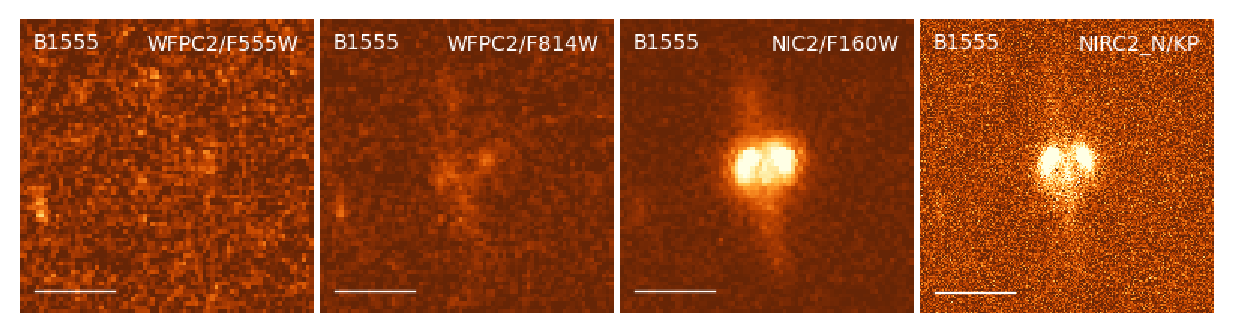
\includegraphics[width=140mm]{B1555_gallery.eps}
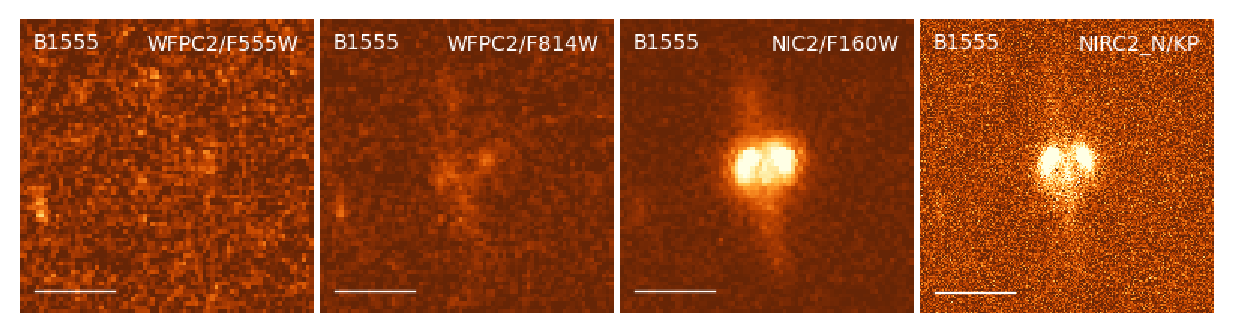
\includegraphics[width=0.95\textwidth]{B1555_gallery.eps}
\caption{High-resolution multiband imaging of the B1555+375 lens system.
All of the panels are 3.7 arcsec on a side, and for each panel the scale bar 
represents 1\arcsec.  From left to right the panels show data from
\textit{HST}/WFPC2 in the F555W band, \textit{HST}/WFPC2 in the F814W band, \textit{HST}/NICMOS/NIC2
in the F160W band, and Keck AO imaging in the $K^\prime$ band.
\label{fig:multiband}}
%
%\end{minipage}

\end{figure*}

\subsection{Keck Adaptive Optics Imaging}

The B1555+375 system was observed using the NIRC2 camera on the Keck 2
Telescope on the night of 2012 May 16 UT.  The adaptive optics system
was used, with the corrections derived from the laser guide star and a
$R$=14.4 tip-tilt \textbf{star} that was located 45 arcsec from the lens
system.  The narrow camera mode was used, giving a field of view
of roughly 10 arcsec on a side and a pixel scale of 10~mas.
Six dithered 300~s exposures were obtained in the $K^{\prime}$ band filter.  The
data were reduced with the standard SHARP pipeline, which is a
python-based package that is a refinement of the process described in
\citet{Auger_EELS1}.  A cutout of the final reduced image is shown in
Fig.~\ref{fig:multiband} and again in Fig.~\ref{fig:merlin} with
contours from the MERLIN radio observations of \citet{Marlow99}
overlaid.  

There are several notable features in the Keck AO data.
These include the nearly complete lack of emission associated with the
B and D lensed images, as can be seen by comparing the radio contours
to the $K^\prime$-band emission, and faint but clearly visible
emission from what appears to be an edge-on lensing galaxy.

\subsection{Hubble Space Telescope Archival Imaging}

The B1555+375 system was also observed with the \textit{Hubble Space Telescope
(\textit{HST})} in three broad bands.  The optical data were obtained with the
Wide-Field Planetary Camera 2 (WFPC2) in the F555W and F814W bands
(GO-8804; PI: E.\ Falco), while the Near Infrared Multi-Object
Spectrograph (NICMOS) was used to observe the system in the $F160W$
band (GO-9744; PI: C.\ Kochanek).  The NICMOS observations were
obtained with the NIC2 camera.  We reduced all of the archival \textit{HST}
data with the standard {\tt multidrizzle} pipeline [?? CHECK WITH
  MATT], producing final drizzled images with pixel scales of 50~mas.
The reduced images are shown in Figure~\ref{fig:multiband}.  The lens
system is not detected at high significance in the optical bands, but
is clearly seen in the NICMOS $F160W$ image \textbf{where the edge-on lensing
galaxy clearly stands out.}
\textbf{The lens system is red, with a strong jump in flux between the F814W
(roughly I) and F160W (roughly H) bands (Fig.~\ref{fig:multiband}), so 
we assign a lens redshift of $z_\ell = 1.0$ and a source redshift of
$z_s =1.5$. This assumption on redshifts is needed for the lens modelling because some lens model parameters contain distance information. However, our choice of redshifts does not affect the predicted magnifications nor flux-ratios.} 

The observation details of Keck AO and \textit{HST} imaging are shown in Table 1.

\begin{table}
 \centering
 %\begin{minipage}{140mm}
  \caption{Observational details of the B1555+375 lens system.}
  \begin{tabular}{@{}llccc}
  
\hline
  Telescope     &      Camera     &  Band & Date &$t_{exp}$ (s) \\

 \hline
   \textit{HST}				&		WFPC2    &  F555W		&	2000/10/09 	&	5200\\
   \textit{HST}				&		WFPC2    &  F814W		&	2000/10/09 &	5200\\
   \textit{HST}				&		NICMOS/NIC2	&	F160W	&	2003/11/02 & 5376\\
   Keck2			&		NIRC2 AO	&   $K^\prime$	& 2012/05/16	&  1800\\
   \hline
\end{tabular}
%\end{minipage}
\end{table}

%===========================================================================

\section{Lens modelling}

%To model B1555+375, we use the lens modelling code {\tt glafic} \citep{Oguri}.  
\textbf{To model B1555+375, we use the lens modelling code {\tt gravlens} \citep{Kee01}.  
The inputs to the model are the observed image
positions and flux densities measured by the radio observations.
We use the image positions from \citet{Marlow99}, who also presented a singular isothermal ellipsoid
(SIE) model that provided a good fit to the image positions but
does not reproduce the strong flux-ratio anomaly between components A
and B.}  %\citep[see Fig.~6 and Tables 2 \& 3 in][]{Marlow99}.  
\textbf{The flux measurements are performed by \citet{K03} with a half year monitoring to obtain flux-ratio curves, providing throughout discussions in erros on flux densities.}

Although the flux-ratio anomaly that is observed in the radio data implies there must be some perturbations to the mass model, which may be
caused by substructure in the lensing galaxy, our high-resolution near
infrared imaging suggests another explanation.  In both the $K^\prime$
band adaptive optics data and the \textit{HST} infrared imaging (see 
Fig. 1), the lensing galaxy has a clear edge-on disk component with a
position angle of $\approx 10$ degree.  We therefore model the system
with a disk component in order to see if such a model can explain the
flux-ratio anomaly without the need for substructure.  The edge-on
disk may also explain the system morphology that is observed in the
near infrared imaging.  In particular, neither image B nor image D is
detected in the Keck AO data (Fig.~\ref{fig:merlin}), and both of
these lensed images lie on or close to the edge-on disk.  Thus, strong
extinction in the disk could cause the non-detection of these
images.[REF B0128 PAPER?--LEON]

As a first trial of modelling, we create a single SIE model to check
the performance of a simple lensing potential. Consistent with
previous studies \citep{Marlow99, Xu14}, a single elliptical
potential model cannot \textbf{reproduce} the flux anomaly in B1555+375.
\textbf{The next step is to examine if an edge-on disk can cause similar perturbations in the strong lensing system  which results in flux ratio anomalies within the merging images. Among most of mass profiles, exponential disk profile best describes the disk component in spiral galaxies because it matches the light distribution of disk \citep{Kee98}. We thus choose a SIE plus exponential disk model (SIE+expdisk) in our study of B1555+375, focusing on the role of its edge-on disk in lens modelling. The free parameters of the model are, SIE: velocity dispersion ($\sigma$), centroid positions, ellipticity ($e$), and position angle ($\theta$); exponential disk: intrinsic central density ($\kappa_0$), centroid positions, ellipticity ($e$), position angle ($\theta$), and scale length ($R_d$). Detail definition of mass profiles in {\tt gravlens} can be found in \citet{Kee01}.}
  We have not included a third component such as an external
shear component or NFW halo into our model because the number of constraints provided by the
image positions and fluxes would not be sufficient to constrain such a
model. However, we note that the image not affected by dust (image C)
in the Keck AO data is consistent with negligible shear (i.e. shear
strength $\Gamma_s=0.002$), when modeled with the pixelized technique
of \citet{V09}.
%We then create two separate models of the lensing potential that both
%incorporate the disk.  In the first we treat the lens as a SIE bulge\textbf{/halo}
%and an exponential edge-on disk (SIE+expdisk). In the second model
%the disk is represented as a very elongated SIE component (2-SIE). 


To obtain \textbf{the minimum $\chi^2$} [OR BEST-FIT MODEL?--JEN] lens model, we explore the parameter space with the following steps: 
\begin{itemize}
\item Preparation of model starting point: Applying the priori infromation from the SHARP AO image, we set ellipticity $e=0.8$ and position angle $\theta=10 \degr$ to the exponential disk. We then use the best-fit model of \citet{Marlow99} as the starting point for the SIE profile and also the source position. The rest of parameters of exponential disk are set to be the same as the SIE component as the starting point.
\item Best-fit model search: We let all model parameter varies but bind the centroid position of two conponents with a Gaussian prior ($\sigma = 0.05 $ arcsec). Run optimization with amoeba algorithm in {\tt gravlens} interatively to reach the global minimum of $\chi^2$ in paramter space.
\item Markov Chain Monte Carlo: After obtaining the best-fit lens model, we run MCMC to explore the parameter space for the uncertainties.
\end{itemize}
%The smallest $\chi^2$ doesn't necessarily give a physical model. Here are the examples we would like to discard: the ellipticity and the position angle of the disk component are far from what we see in the SHARP AO image, the center positions of two components are too far apart physically, or the positions of the lenses and the source are clearly located outside the Einstein radius in the image.
%(3) Optimize for physical lens models: We bind the positions of the two components with a strong Gaussian prior having the same central position and $\sigma = 0.05 $ arcsec and then run optimization with amoeba algorithm to reach the final best-fit for each model.}  

The best-fit model parameters are listed in Table 2 and the lens model is illustrated in Fig. 3. 
%Both of these models produce lensed images with positions and
%fluxes that are good matches to the radio observations.  
%While both of the two component models 
%the 2-SIE version has a somewhat
%better performance than the SIE+expdisk model in reproducing flux
%ratios. 
Tables 3 \& 4 show the comparison between radio data and model predicted image positions and flux ratios.  
\textbf{By adding an elongated exponential disk to a smooth potential model, the SIE+expdisk lens model shows significant improvement on the flux ratios when comparing to the SIE-only model, especially the flux ratio anomaly between the merging images.}


\begin{figure}
%\plotone{1555_ao_merlin_overlay.eps}
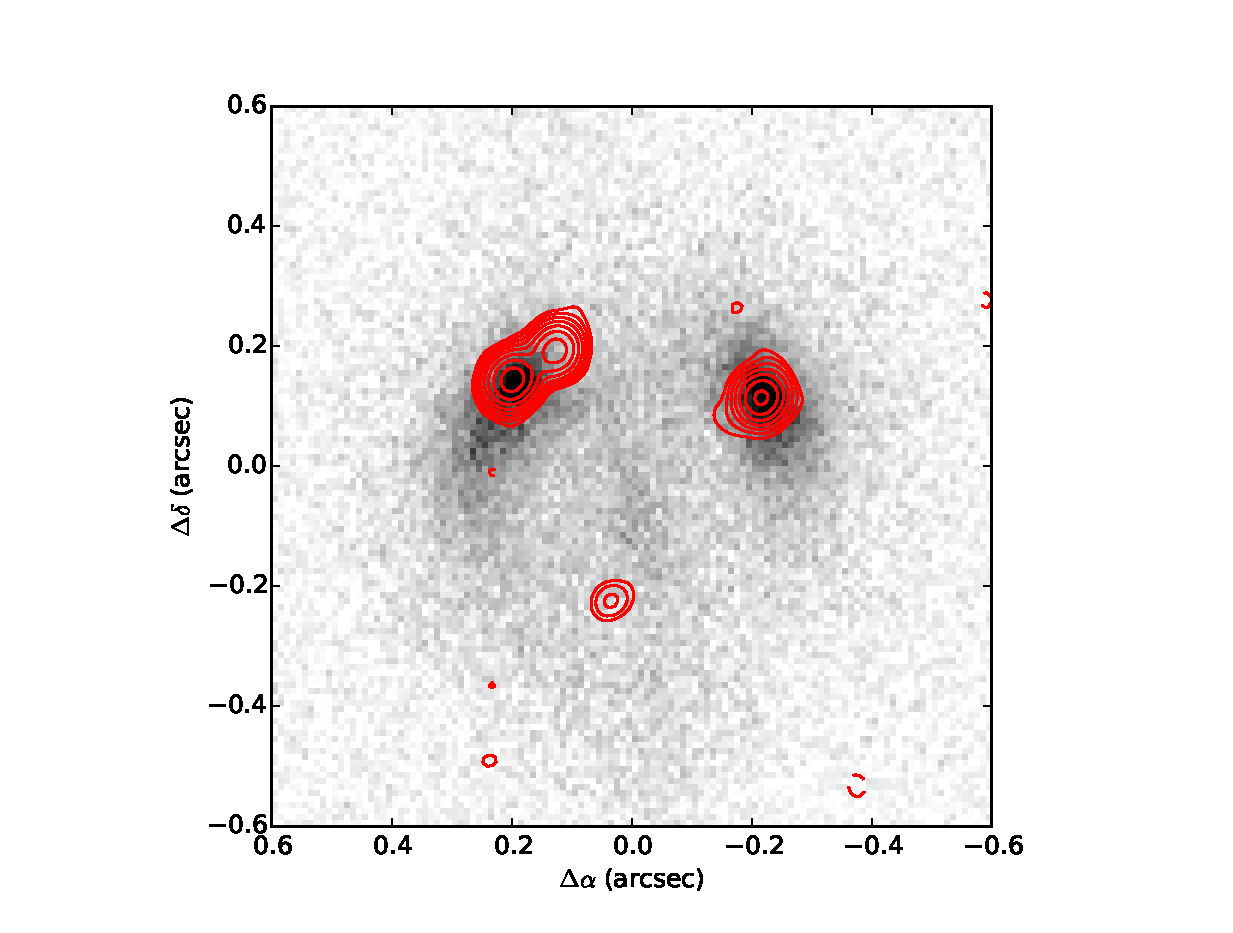
\includegraphics[width=84mm]{1555_ao_merlin_overlay.eps}
\caption{High-resolution  $K^\prime$ band imaging of the B1555+375 lens system 
with contours from the MERLIN observation of \citet{Marlow99} overlaid. 
%
\label{fig:merlin}}
\end{figure}


\begin{figure}
%\plotone{point_source.eps}
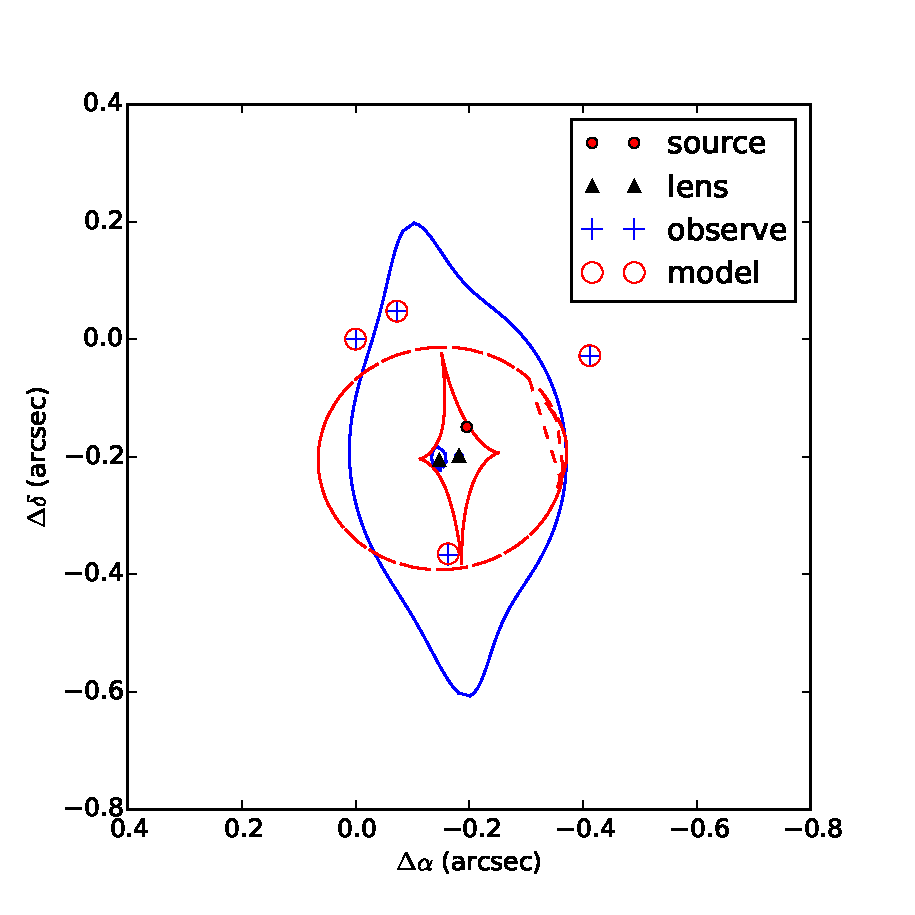
\includegraphics[width=84mm]{gravlens_exp_try5_plot.eps}
\caption{Radio observation(blue plus sign) and model-predicted(red open circle) image positions of B1555+375. Criticle curves are shown with blue solid line and caustics are shown with red dash line. The position of the source is at $(-0.1953,-0.1494)$, marked by a red filled circle. The centroid positions of two lens components are marked by black filled triangles.  \label{fig2}}
\end{figure}

%\begin{figure}
%\plotone{point_source.eps}
%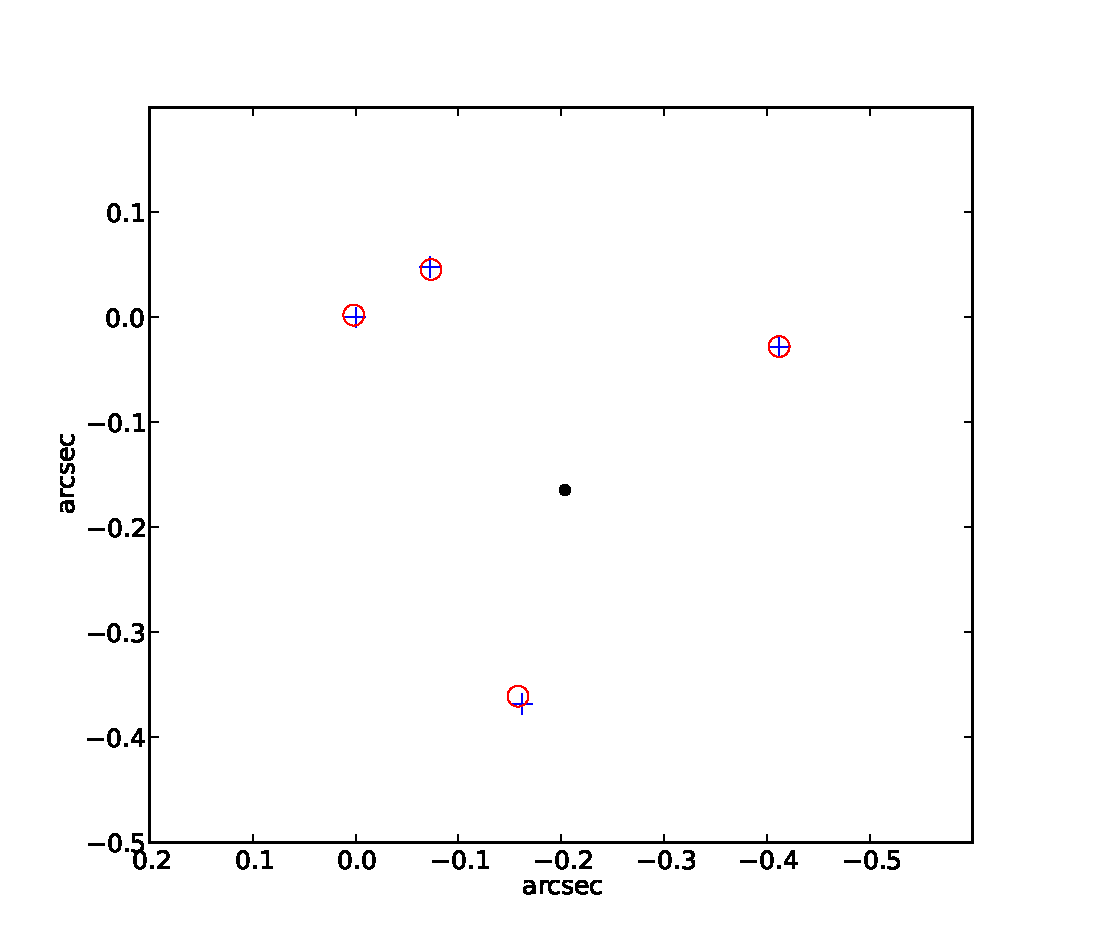
\includegraphics[width=84mm]{point_source.eps}
%\caption{Radio observation(red open circle) and model-predicted(blue plus sign) image positions of B1555+375. The position of the source is at $(-0.2066,-0.1634)$ for SIE+Expdisk model [NOT UPDETED YET], marked by a black filled circle. \label{fig2}}
%\end{figure}

\begin{table}
 \centering
% \begin{minipage}{140mm}
  \caption{Best-fit parameters of B1555+375 SIE+expdisk lens model and uncertainties. Positions are offsets from radio image component A measured in units of arcsec. The velocity dispersion $\sigma$ is in units of $km/s$. \textbf{$e$ is ellipticity defined as the axis ratio $q=1-e$ }and $\theta$ is the position angle measured east of north.}
  \begin{tabular}{@{}ccc}
\hline 
 Parameter  & SIE & Expdisk 		   
\\
\hline
$x$  	  & $-0.1818 \pm 0.005$	&$-0.1472 \pm 0.005$ 	  \\
$y$	  &$-0.1988 \pm 0.005$	&$-0.2057 \pm 0.006$	 \\

$b$ &$0.21 \pm 0.01$  & ...   \\
$\kappa_0$ & ... & $0.11 \pm 0.01$        \\  
$e$	  & $0.31\pm 0.01$	&$0.87 \pm 0.01$ \\
$\theta$ &$2.96 \degr \pm 0.64 \degr$ &$7.00\degr \pm 0.70 \degr$ \\
$R_s$	& ...  & $0.28 \pm 0.01$\\
\hline
%$\chi ^2$ & $1.05$ & $0.04$ \\
%\hline
\end{tabular}

%\end{minipage}
\end{table}

%\begin{table}

%  \caption{Best-fit parameters of B1555+375 lens models. Subscripts 1 and 2 represent bulge\textbf{/halo} and disk components in each model respectively. Positions are offsets from radio image component A measured in units of arcsec. The velocity dispersion $\sigma$ is in units of $km/s$ and disk mass $M_{tot}$ is in units of $h^{-1} M_{\odot}$. \textbf{$e$ is ellipticity defined as the axis ratio $q=1-e$ }and $\theta$ is the position angle measured east of north.}
%  \begin{tabular}{@{}ccc}
%\hline 
% Parameter  & \multicolumn{2}{c}{Lens model} \\
%		&SIE+expdisk& 2-SIE		   
%\\
%\hline
%$x_1$  	  & $-0.1794$	& $-0.1771$  \\
%$y_1$	  &$-0.1881$	&$-0.2032$  \\

%$\sigma_1$ &$140.3$     & $146.1$ \\
%$e_1$	  & $0.21$	& $0.15$ \\
%$\theta_1$ &$73.6 \degr$ & $155.3 \degr$ \\
%\hline
%$x_2$	  &$-0.1639$ 	&$-0.1562$  \\
%$y_2$	  &$-0.2542$	& $-0.2195$  \\
%$M_{tot,2}$  & $3.58\times 10^{10} $  & ...	 \\  
%$\sigma_2$ & ...        &$122.6$ \\  
%$e_2$	  &$0.84$	&$0.86$  \\
%$\theta_2$ &$4.0\degr$ &$7.9\degr$  \\
%$r_e$	  & $0.21 ''$ &  ... \\
%\hline
%$\chi ^2$ & $1.05$ & $0.04$ \\
%\hline
%\end{tabular}
%\end{table}

%\begin{table*}
\begin{table}
\centering
 %\begin{minipage}{140mm}
  \caption{Radio observation \citep{Marlow99} and model-predicted lensed image positions (in arcsec). Uncertainties in position measurements are $0.001^ {\prime \prime}$ expect image D with larger uncertainty ($0.006^ {\prime \prime}$).}
  \begin{tabular}{@{}ccccc}
\hline

Component	&\multicolumn{2}{c}{MERLIN} 	 & \multicolumn{2}{c}{Model} \\
					&\multicolumn{2}{c}{5 GHz}		&	\multicolumn{2}{c}{SIE+expdisk} 	\\
					 &East &North &East 		&North \\ 
\hline
A ........ &$0$    		&$0$		&$0.0000$ &$0.0000$   \\  
B ........ &$-0.0726$ 	&$+0.0480 $	&$-0.0727$ &$+0.0477$  \\  
C ........ &$-0.4117$  &$-0.0280$	&$-0.4117$ &$-0.0281$   \\  
D ........ &$-0.1619$  &$-0.3680$	&$-0.1630$ &$-0.3653$  \\  
%A ........ &$0$    		&$0$		&$0.0000$ &$0.0000$   \\  
%B ........ &$-0.0726\pm 0.001$ 	&$+0.0480 \pm 0.001$	&$-0.0727$ &$+0.0477$  \\  
%C ........ &$-0.4117\pm 0.001$  &$-0.0280 \pm 0.001$	&$-0.4117$ &$-0.0281$   \\  
%D ........ &$-0.1619\pm 0.006$  &$-0.3680\pm 0.006$	&$-0.1630$ &$-0.3653$  \\  
\hline
\end{tabular}

%\end{minipage}
%\medskip
\end{table}
%\end{table*}

%\begin{table*}
%\centering
 %\begin{minipage}{140mm}
 % \caption{Radio observation \citep{Marlow99} and model-predicted lensed image positions (in arcsec). Both SIE+expdisk and 2-SIE lens model-predicted positions well match to the radio observation.}
 % \begin{tabular}{@{}ccccccc}

%\hline

%Component	&\multicolumn{2}{c}{MERLIN} 	 & \multicolumn{4}{c}{Model} \\
%					&\multicolumn{2}{c}{5 GHz}		&	\multicolumn{2}{c}{SIE+expdisk} &\multicolumn{2}{c}{ 2-SIE}		\\
%					 &East &North &East 		&North &East 		&North\\ 
%\hline
%A ........ &$0$    		&$0$		&$0.0000$ &$0.0000$   &   $0.0000$   &  $ 0.0000$\\  
%B ........ &$-0.0726(0.001)$ 	&$+0.0480(0.001)$	&$-0.0723$ &$+0.0480$ & $-0.0755 $  &  $+0.0414$  \\  
%C ........ &$-0.4117(0.001)$  &$-0.0280(0.001)$	&$-0.4114$ &$-0.0282$  & $-0.4122 $  &   $-0.0267$ \\  
%D ........ &$-0.1619(0.006)$  &$-0.3680(0.006)$	&$-0.1631$ &$-0.3628$  & $-0.1620$    &  $-0.3533$ \\  
%\hline
%\end{tabular}

%\end{minipage}
%medskip
%\end{table*}

\begin{table}
 \centering
% \begin{minipage}{140mm}
  \caption{Comparison between radio data \citep{K03} and model-predicted flux-ratios from SIE-only and SIE+expdisk model.}
  \begin{tabular}{@{}ccccccc}

\hline
	& MERLIN  & \multicolumn{2}{c}{Model}\\
		&5 GHz   & SIE-only & SIE+expdisk \\
\hline
$f_A/f_B$			&$1.61 \pm 0.10$ &$1.04$& $1.62$  \\ 
$f_A/f_C$		&$1.97 \pm 0.12$ 	 &$3.20$ & $2.17$ \\
$f_A/f_D$		&$11.62 \pm 3.24 $  &$9.67$& $8.69$ \\

\hline
\end{tabular}

%\end{minipage}
\medskip
\end{table}

%\begin{table}
% \centering
% \begin{minipage}{140mm}
%  \caption{Comparison between radio data \citep{K03} and model-predicted flux-ratios.}
% \begin{tabular}{@{}ccccccc}

%\hline
%	& MERLIN  & \multicolumn{3}{c}{Model}\\
%		&5 GHz   & 1-SIE & SIE+expdisk & 2-SIE\\
%\hline
%$f_A/f_B$			&$1.61 (0.10)$ &$1.04$& $1.62$ & $1.62$ \\ 
%$f_A/f_C$		&$1.97 (0.12)$ 	 &$3.20$ & $2.89$ & $2.00$\\
%$f_A/f_D$		&$11.62 (3.24)$  &$9.67$& $9.30$ & $11.56$\\

%\hline
%\end{tabular}

%\end{minipage}
%\medskip
%\end{table}

\section{Discussion}

Gravitational lensing is, at present, the most powerful tool for
studying substructure in galaxies outside of the Local Universe, and
the flux-ratio anomaly systems are a key aspect of these
investigations.  However, before using the anomaly in any
given system to investigate structure formation and the properties of
dark matter, it is critical to eliminate other possible explanations
for the difference between the observed and expected fluxes, such as
propagation effects and assumptions about the lens galaxy's mass distribution.  
It is for this reason that much of the effort in the
flux-ratio technique has been focused on radio-loud lens systems.  At
these wavelengths, dust extinction and microlensing effects should be
minimal \citep[although see][for a rare example of radio
  microlensing]{K2000}.  \textbf{Also,  scatter broadening} can affect radio
fluxes, as is clearly shown in the B0128+437 system \citep{B04}, and free-free absorption can change the flux-ratios as a function of frequency,
for example, B0218+357 \citep{M07}.
However, these propagation effects can be disentangled from
substructure lensing because they have well known dependencies on
wavelength. In particular, \citet{KD04} examine all eight radio-loud flux anomalous
lenses besides B0128+437, namely: MG 0414+0534, B0712+472, B1359+154,
B1422+231, B1555+375, B1608+656, B1933+503, and B2045+265.  They find
no strong wavelength dependence in the flux-ratios of all these
systems and therefore rule out radio propagation effects as
significant contributors to the observed anomalies.

In this letter, we \textbf{instead} focus on the effect that more complicated lens galaxy mass
distributions \textbf{have} on flux-ratio anomalies.
Traditionally, flux-anomalous lensed quasars \textbf{have been} radio-loud, initially discovered in radio observations. While radio data
provide reliable information on the positions and the fluxes of the
lensed images, they are often unable to detect the lens
galaxies. Moreover, lens modelling based only on the positions of the
four images can be highly degenerate and prior assumptions play a key
role in the interpretation of the observed flux-ratio anomaly.  Since
lens galaxies are typically at redshifts of $z \leq 1$, optical and
near-infrared observations are ideal for measuring the light distribution
of lens galaxies and obtaining useful prior information on the underlying
mass distributions. Indeed \citet{SHARP12} showed that high
resolution IR imaging can help to significantly improve the precision
of the lens modelling. This improvement is even more dramatic in the
case of B1555+375, where \textit{HST} and SHARP AO high resolution imaging has
allowed us to detect, for the fist time, the presence of an edge-on
disk. This newly discovered edge-on disk provides a strong prior for our
lens modelling.  With an additional disk component, our model 
matches to both the radio image positions and their flux-ratio, wheras
models with only one SIE component \citep{Marlow99,Xu14} fail to
reproduce the fluxes correctly. Our successful modelling indicates
that the kiloparsec-scale structure of the lens galaxy itself is
sufficient to explain the flux-ratio anomalies in B1555+375, without
any need to invoke the presence of substructure.

From a theoretical perspective, \citet{Xu14} also find that substructures
cannot explain the observed radio flux anomalies in all the lenses
that were considered. After adding subhaloes from numerical simulations
to these systems, only one out of the eight radio-loud systems
achieves the level of the flux anomalies seen in the observations.  The rest of
them are unlikely (only $1 - 4$ per cent probability) to have \textbf{observed distribution of flux
anomalies} produced only by substructure, including our target B1555+375.
In fact, among those eight radio lenses, B1555+375 is one of the most
anomalous systems, but it is also one of the most challenging systems
to explain by substructures. \citet{Xu14} have concluded that the failure in
predicting flux-ratios is most likely due to oversimplified/improper lens
modelling. They also point out that the SIE component and the external
shear in their model are orthogonal, indicating a possible missing
ingredient in the lens model.
\textbf{Indeed, it's hard to find physical interpretation for an large and orthogonal external shear.
The SHARP $K^{\prime}$ band observations provide another explaination to their result. The edge-on disk crosses the
radio merging double is consistent of this missing component and fully accounts for the observed flux-ratio anomaly.} 
In general, it is well known  \citep[e.g.][]{Ka91} that lens models based only on the locations of lensed
quasar/AGN images have large degeneracies. Therefore, before
concluding that the flux-ratios in any given lens system are a result
of substructure, it is critical to explore a range of smooth models
that are informed by additional observations or to do a comprehensive
analysis such as that conducted by \citet{Xu14}. Otherwise, the derived
substructure fractions should be considered as upper limits.
 
%Although the number of radio-loud flux anomalous lensed
%quasars remains small, a new technique using narrow-line emission
%regions will enlarge the sample and bring statistical perspective on
%substructures in the near future \citep{N14}. 

\section{Conclusions}
In this letter we have taken advantage of the power of
multi-wavelength high resolution data to investigate whether flux
ratio anomalies could be explained by more complex smooth models for
the lens galaxy mass distribution rather than substructure. Thanks to
new imaging from the SHARP $K^{\prime}$ band observations of the
gravitational lens system B1555+375, we have identified the existence
of a previously unknown edge-on disk. By including this disk in the
mass model of the lens galaxy, we find a good fit for both the
positions and flux-ratios of the lensed images. 

Our results clearly
demonstrate that the lack of knowledge on the lens galaxy mass
distribution, combined with the limited information provided by the
position of a few lensed images, can lead to improper lens models and
a misinterpretation of the origin of flux-ratio anomalies. \textbf{While upcoming large-scale surveys, such as the DES, KiDS-VIKING, Euclid, and LSST, are expected to
deliver new large samples of gravitationally lensed quasars, in the
near future the discovery of new systems using narrow-line quasar
emission \citep{N14} will provide new invaluable statistical
perspective on current constraints based on flux-ratio anomalies.} We stress,
therefore, that one should be very careful when interpreting the
nature of flux-ratio anomalies, as prior assumptions on the lens mass
distribution are a significant source of bias. Our analysis shows that
in order to derive precise quantification of the substructure
population and any derived properties from strongly lensed flux
anomalous systems, it is crucial to have a careful estimation of
non-substructure effects. In fact, even in the presence of mass
substructures, the observed flux-ratio anomalies could be still
dominated by the complex structure of the lens galaxy. Finally,
additional near-infrared AO imaging from SHARP shows that B1555+375 is
not the only system having a significant disk component detection in
the lensing galaxy.  These systems will be investigated in future
work, but the images alone strongly suggest that other lens systems
have similar links between flux-ratio anomalies and disk components.


%. modelling with only four image positions from radio data can also cause a lot of degeneracy. With the first system analyzing and finding an edge-on disk originated flux-ratio anomaly, our follow up will be explore other similar SHARP systems. In Figure 3, all of these systems have a recognizable edge-on disk in infrared imaging. An edge-on disk structure may also be able to explain the flux-ratio anomalies of these systems.
 %From the successful modelling of B1555+375,  we expect more flux anomalous systems requiring complex lens models (e.g. include an exponential disk), rather than just assuming smooth potential. Although the number of radio-loud flux anomalous lensed quasars remains small, a new technique using narrow-line emissions will enlarge the sample and bring statistical perspective on substructures in the near future \citep{N14}. If the non-substructure effect from edge-on disks does not included, expected ``false'' substructure detections can serverly bias the data analysis. 
% This breaks the idea that in strongly lensed quasars, radio flux-ratio
% anomalies are most likely originated from substructure
% perturbations. Our discovery shows a complex lens galaxy mass
% distribution can dominate flux-ratio anomalous phenomena in a strongly
% lensed system.
% We would like to draw attention to the possible impacts on
% substructure searching from this enge-on disk orginated flux
% anomalies. It is a sign that researchers should be careful about the
% flux anomalies fraction in lensed quasars. It may be worth considering
% an upper limit of flux anomalies fraciton from observation results to
% avoid over estimate the number of substructure detections. For further
% analysis on substurcture population, mass function etc., it is always
% important to rule out other non-substructure effects.

\section*{Acknowledgments}
S.V. is grateful to Dandan Xu for useful discussion.
L.V.E.K. is supported in part through an NWO-VICI career grant (project number 639.043.308).
\bibliographystyle{mn2e}
\bibliography{reference.bib}




\label{lastpage}

\end{document}
